\chapter{Parametrising the speed distribution}
\label{ch:Speed}

As we have explored in Chapter~\ref{ch:DD}, there are a number of uncertainties associated with calculating the direct detection event rate. These translate directly into uncertainties in the analysis of direct detection results, present and future. If these uncertainties are properly accounted for, they can provide a more realistic estimates of uncertainties on the WIMP cross sections \sigmapsi and \sigmapsd and WIMP mass \mchi. If, however, our assumptions do not reflect the underlying nuclear physics, particle physics or astrophysics of dark matter, this can lead to a bias in the WIMP parameters. Understanding these uncertainties and how to mitigate them is therefore of great importance.

The WIMP speed distribution $f(v)$ enters into the direct detection event rate as it influences both the typical flux of dark matter particles and the typical recoil energy imparted during a scattering event. Unfortunately, the typical flux and recoil energy are also strongly dependent on the WIMP mass \mchi. This leads to a strong degeneracy between \mchi and $f(v)$ and, as discussed in Sec.~\ref{sec:DD:astrophysics}, the possibility of significant bias in the reconstruction of the WIMP mass (see e.g. Ref~\cite{Peter:2011}). \note{Maybe move some of the DD background chapter stuff to here...} In Sec.~\ref{}, we revisit the problem of reconstructing the WIMP mass and how it can be influenced by poor assumptions about $f(v)$.

Because the speed distribution is so poorly constrained, an ideal goal would be to construct the most general parametrisation for $f(v)$ which can accommodate a wide range of possibilities for the true functional form. This approach has previously been explored by Peter \cite{Peter:2011}, who wrote down an empirical parametrisation for $f(v)$ as a series of constant bins in $v$. However, this still resulted in a bias in the reconstructed WIMP parameters. In Sec.~\ref{sec:Speed:binned}, we analyse in more detail the performance of this method and attempt to explain where this bias comes from.

In Sec.~\ref{sec:Speed:momentum}, we discuss a method analogous to that of Peter but for parametrising the WIMP \textit{momentum} distribution in terms of a series of constant bins. This transformation helps remove some of the degeneracy between the WIMP mass and distribution function and improves reconstructions of the mass compared to binning in $f(v)$. However, this method is not generally applicable and begins to fail for low mass WIMPs.

%In Sec.~\ref{sec:Speed:poly}, we propose an alternative parametrisation. Instead of parametrising $f(v)$, we parametrise the logarithm of $f(v)$ as a series of polynomials. This permits the most general possible form from $f(v)$ satisfying the constraint $f(v) \geq 0$. We demonstrate the performance of this new method over a range of WIMP masses and over a range of underlying speed distributions and experimental parameters. We show that this method allows us to reconstruct the WIMP mass without bias, as well as allowing us to reconstruct information about the WIMP speed distribution itself. \note{What about doing some 1-D plots for $f(v)$ parameters, such as plotting $\langle v \rangle$ or similar...?}

Finally, we compare these different parametrisations in Sec.~\ref{sec:Speed:discussion} and discuss how they relate to alternative methods of accounting for astrophysical uncertainties in direct detection experiments. We will also discuss the weaknesses of the momentum parametrisation, highlighting where remaining work is needed.

\section{Uncertainties in $f(v)$}
\label{sec:Speed:uncertainties}

Dark matter direct detection experiments simultaneously probe the WIMP speed distribution and WIMP mass. As described in Chapter~\ref{ch:DD}, the differential event rate relevant for direct detection experiments is

\begin{equation}
\dbd{R}{E_R} = \frac{\rho_0}{2 \mu_{\chi p}^2 m_x} \sigma_{SI}^p A^2 F_{SI}^2(E_R) \int_{v_\textrm{min}}^\infty \frac{f(v)}{v}\,\mathrm{d}v\,,
\end{equation}
where for simplicity we have assumed that the coupling to protons and neutrons is the same ($f_p \approx f_n$) and we consider only the spin-independent (SI) contribution to the rate. Not also is the SI contibution expected to dominate for heavy nuclei (due to the $A^2$ enhancement), but considering only a single contribution allows us to focus on the degeneracies between \mchi, \sigmapsi and $f(v)$.

We have previously outlined in Chapter~\ref{ch:DD} that there are various possibilities for the form of the WIMP speed distribution and that poor assumptions about this form may lead to biased reconstructions of the WIMP parameters. This has been demonstrated, for example, by Peter \cite{Peter:2011}, who attempted to reconstruct the WIMP mass and SI cross section from mock data sets based on future direct detection experiments. In order to generate the data, an SHM distribution function with an additional contribution from a dark disk was assumed. However, the posterior distribution for \mchi and \sigmapsi was obtained assuming that $f(v)$ could be well described by a single Maxwell-Boltzmann (MB) distribution (with average speed and speed dispersion included as nuisance parameters). The resulting marginalised 68\% and 95\% contours for \mchi and \sigmapsi are shown in Fig.~\ref{fig:Speed:PeterRecon}, with the true parameter values given by the black crosses.

\begin{figure}[h]
  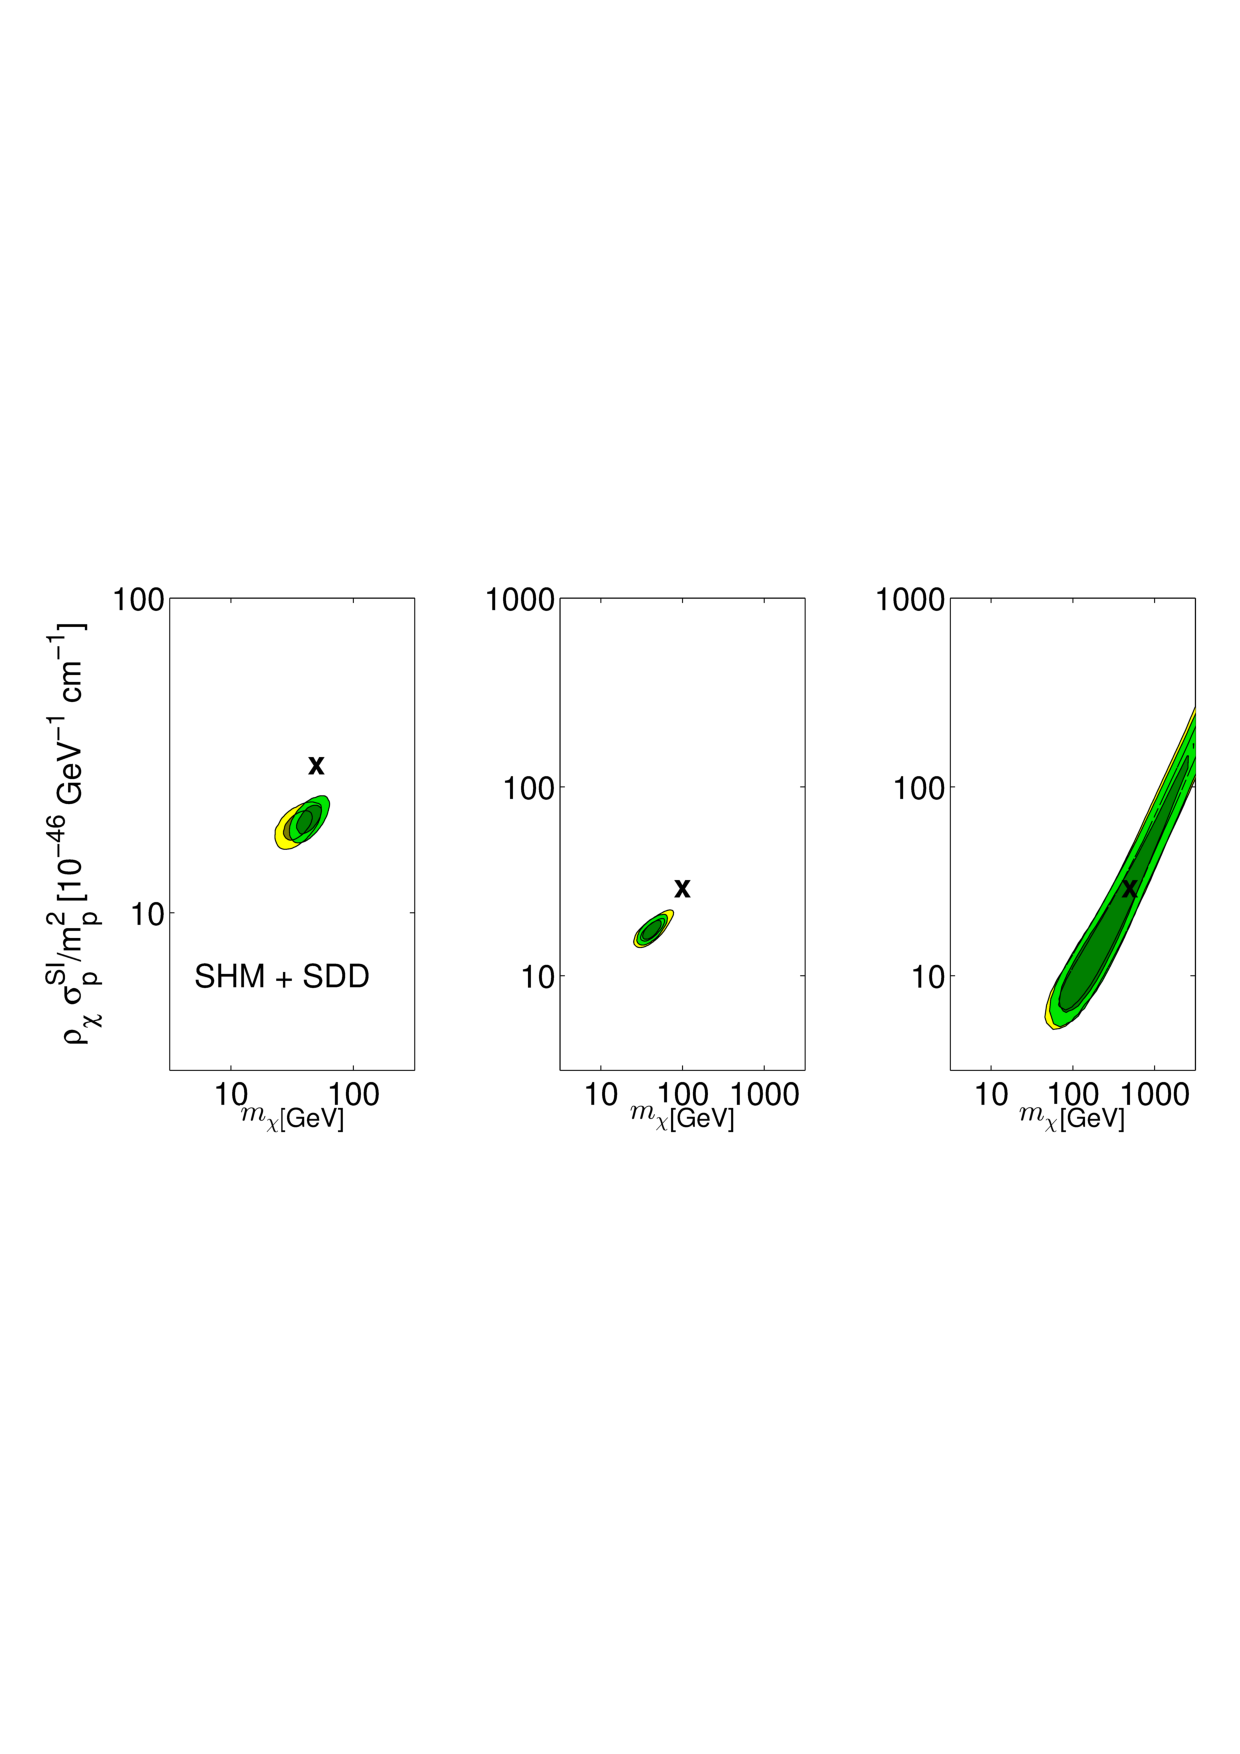
\includegraphics[trim={0cm 9cm 0cm 9cm},clip,width=\textwidth]{Speed/PeterRecon.pdf}
  \caption[Biased reconstruction of WIMP parameters]{\note{Need caption...} Reproduced from Ref.~\cite{Peter:2011}}
  \label{fig:Speed:PeterRecon}
\end{figure}

Even including some uncertainties in the shape of the MB speed distribution, there is still a clear bias in the reconstructed WIMP parameters. The MB speed distribution cannot reproduce the shape of the event spectrum closely and the WIMP mass and cross section move to different values to compensate and improve the fit. Not only is there a bias, but the resulting contours are relatively small. In this case, if we trust the ansatz of a MB distribution, we would mistakenly believe that we had reconstructed the WIMP parameters accurately with a high precision. Thus, there is a need for a more general approach which allows a broad range of speed distributions to be probed. We discuss the consequences of such an approach now. \todo{Improve flow...}

We can write the integral over the speed distribution as
\begin{equation}
\label{eq:Speed:eta}
\eta(\vmin) \equiv \int_{\vmin}^\infty \frac{f(v)}{v}\,\mathrm{d}v\,,
\end{equation}
where \vmin is given by
\begin{equation}
v_\textrm{min} = v_\textrm{min}(E_R, \mchi, m_N) = \sqrt{\frac{m_N E_R}{2 \mu_{\chi N}^2}}\,.
\end{equation}
If we treat $f(v)$ as a free function (subject to the condition that it be normalised to unity and everywhere positive), this is equivalent to treating $\eta(\vmin)$ as a free function (subject to the equivalent condition that $eta$ be a monotonically decreasing function of \vmin). This represents an entirely agnostic approach to $f(v)$, assuming that we know nothing at all about its functional form. Unfortunately, if we fix $m_N$, any change in the form of $\eta$ can be counteracted by a change in $\mchi$ (and a resulting change in \vmin) leading to the same spectral shape $\eta(E_R)$. This means that for a single experiment, the WIMP mass and $f(v)$ are exactly degenerate and we need multiple experiments to disentangle the two \cite{Drees:2008}. We will phrase this in more concrete terms later in Sec.~\ref{sec:Speed:momentum}.

Another consideration when parametrising $f(v)$ is the range of sensitivity of the experiments. Each experiment will have a window recoil energies to which it is sensitive $\left[\Emin, \Emax\right]$ (though the recoil detection efficiency may vary across this window). This means that for a given WIMP mass, each experiment will be sensitive only a range of WIMP speeds $\left[\vmin(\Emin), \vmin(\Emax)\right]$. WIMPs with speeds smaller than $\vmin(\Emin)$ do not contribute to the velocity integral defined in Eq.~\ref{eq:Speed:eta}. WIMPs with speeds above $\vmin(\Emax)$ can contribute to the overall spectrum, but they contribute only a constant, additive rate; the experiment is not sensitive to the \textit{shape} of the speed distribution above this maximum speed. Thus, each experiment has a range of speeds to which it is sensitive. If we wish to probe the shape of $f(v)$, these ranges must have some overlap between the different experiments. Otherwise, the $f(v)$ can be varied independently across each speed range and the degeneracy between \mchi and $f(v)$ remains. \todo{Insert and explain plot...}

In order to get a handle on $f(v)$ and therefore the WIMP mass we therefore need several direct detection experiments, which use different target materials but which probe overlapping WIMP speeds. However, we must come up with a way of writing our general function $f(v)$ which allows us to reconstruct it by fitting to the data. Such a parametrisation should correspond to a physical distribution function; it should be normalised and should be everywhere positive. We should try to write down a parametrisation which spans a wide range of underlying distribution functions and which does not introduce any additional bias into attempts to reconstruct the WIMP parameters. For this reason, it is necessary to carefully test any proposed parametrisation. We now explore in more detail several proposal for what such a general parametrisation should look like.

\todo{Talk about the transformation from the Galactic to Earth frame...}

\section{Binned speed distribution}

Peter proposed using an empirical speed distribution in the form of series of bins in speed $v$ in order to fit to data. Explicitly, we write the WIMP speed distribution (in the Earth frame), as a series of \(N\) bins of constant value, with bin edges \(\{ \tilde{v}_i\}\): \note{This is the directionally averaged velocity distribution...}

\begin{equation}
\label{eq:Speed:binned}
f(v) = \sum_{i = 1}^N g_i \, W(v;\tilde{v}_i,\Delta v) \,,
\end{equation}
where the top-hat function, W, is defined as:

\begin{equation}
W(v;\tilde{v}_i,\Delta v) =
\begin{cases}
   1 &  v \in [\tilde{v}_i,\tilde{v}_i+\Delta v] \\
   0  & \text{otherwise}
  \end{cases} \,.
\end{equation}
We must choose a maximum speed $v_\textrm{max} = N\Delta v$ up to which we parametrise. Beyond this speed, we set $f(v)$ to zero, so we should choose a conservative value which does not risk truncating the speed distribution prematurely. Based on the results of the RAVE surveys \cite{RAVE:2007, RAVE:2014}, the Galactic escape speed is estimated to be $\vesc < 587$ at the 90\% confidence level. Assuming a local circular speed of $v_c \sim 220 \kms$ \cite{Kerr:1986,Feast:1997}, this means that in the Earth frame, particles with speeds significantly higher than $v_c + \vesc \sim 800 \kms$ should not be gravitationally bound. This is consistent with results for the local escape speed obtained in N-body simulations \cite{Kuhlen:2010}. We therefore choose a value $v_\textrm{max} = 1000 \kms$ as a conservative upper limit for the parametrisation.

The form for the distribution function given in Eq.~\ref{eq:Speed:binned} is the directionally-averaged WIMP velocity distribution, $f(v)$. The WIMP \textit{speed} distribution is then given by

\begin{equation}
\label{eq:Speed:binned2}
f_1(v) = \sum_{i = 1}^N g_i v^2\, W(v;\tilde{v}_i,\Delta v) \,.
\end{equation}
Imposing normalisation of the speed distribution, we obtain the following constraint on the \(\{g_i\}\):
\begin{equation}
\label{eq:Speed:Normg}
\sum_{i = 1}^N g_i \, \left[(\tilde{v}_i + \Delta v)^3 - \tilde{v}_i^3\right]/3 = 1 \,.
\end{equation}
For notational convenience, we also define
\begin{equation}
\hat{g}_i = g_i \, \left[(\tilde{v}_i + \Delta v)^3 - \tilde{v}_i^3\right]/3 \,,
\end{equation}
such that the normalisation condition becomes
\begin{equation}
\label{eq:Speed:ghat}
\sum_{i = 1}^N \hat{g}_i = 1.
\end{equation}
\todo{Distinguish between f1 and f...}

\todo{Earth frame}

We illustrate the form of this binned distribution for $f(v)$ in Fig.~\ref{fig:Speed:BinApprox}. We show the Standard Halo Model in the Earth frame (blue line) as well as the binned approximation to the SHM (red line). This approximation is obtained by integrating the WIMP speed distribution over each of the bins:

\begin{equation}
\label{eq:Speed:gapprox}
\hat{g}_i^\textrm{approx} = \int_{\tilde{v}_i}^{\tilde{v}_i + \Delta v} f_1^{\textrm{SHM}}(v) \, \mathrm{d}v\,.
\end{equation}
This allows us to examine how closely the binned parametrisation can be used to approximate the SHM. However, in a realistic scenario, these bin parameters $\left\{\hat{g}_i\right\}$ would form part of the parameter space, along with \mchi and \sigmapsi, which must be explored based on the data. \note{Also plot the approximate form for $\eta$ here!}

\begin{figure}[h]
\centering
  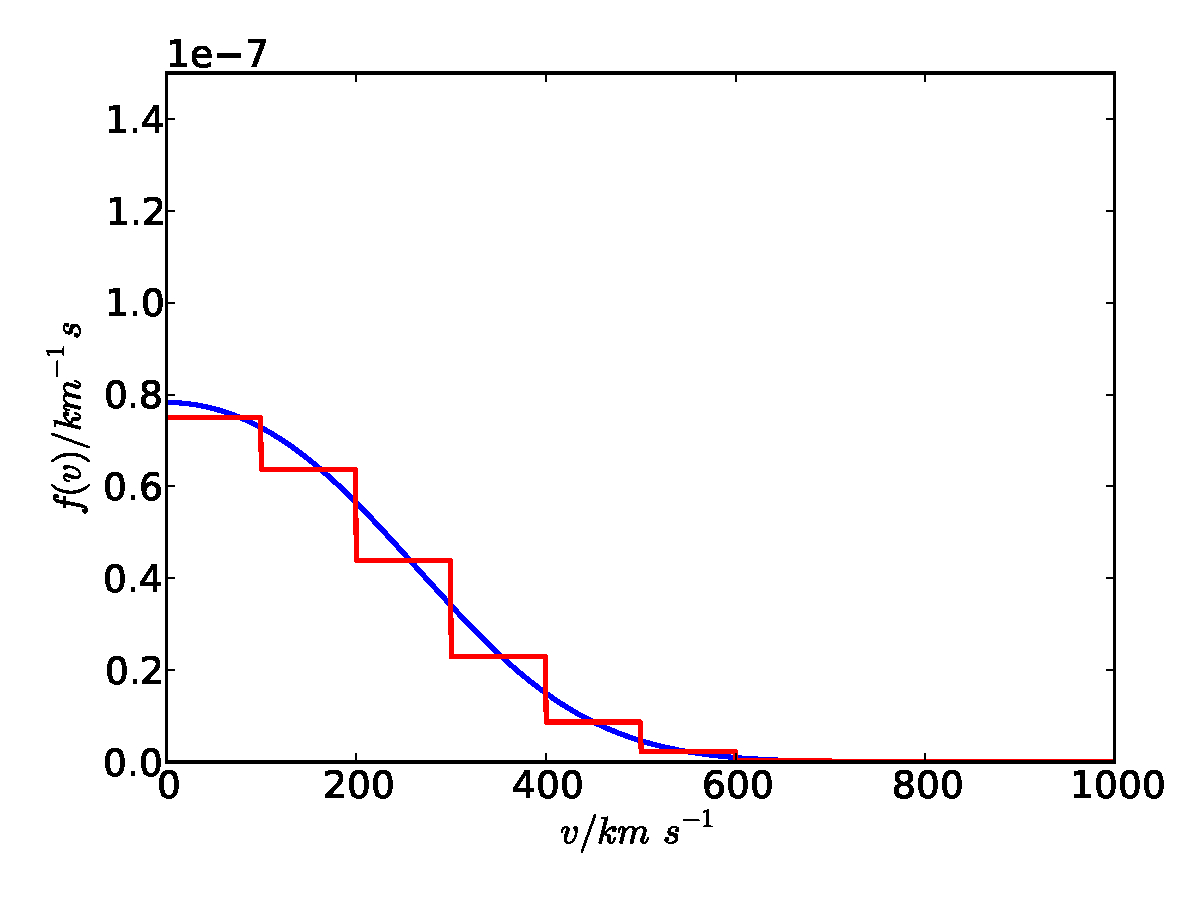
\includegraphics[width=0.75\textwidth]{Speed/BinnedApprox.pdf}
  \caption[Binned approximation to the SHM]{Binned approximation to the SHM in the Earth frame. The bin heights are obtained from Eq.~\ref{eq:Speed:gapprox}. We note that shown here is $f(v)$, the directionally-averaged velocity distribution. We must multiply by $v^2$ to obtain the speed distribution $f_1(v)$.}
  \label{fig:Speed:BinApprox}
\end{figure}

In Ref.~\cite{Peter:2011}, Peter found evidence that this method still lead to a bias in the reconstructed WIMP mass and cross section, despite the apparent generality of this binned distribution function. Here, we explore this method further. In particular, we consider a large number of realisations of data sets from hypothetical future experiments, assuming some fiducial benchmark model. We then attempt to reconstruct the WIMP mass for each realisation, allowing us to determine how the method performs statistically and whether the bias found by Peter is present in all data sets or only in a small number of Poissonian realisations.

\subsection{Benchmark Parameters and Experiments}
\label{sec:Speed:Experiments}
As noted in Sec.~\ref{sec:Speed:uncertainties}, it is impossible to estimate the WIMP mass from a single experiment if no assumptions are made about \(f(v)\), so we consider three next-generation detectors, modelled on experiments which are currently in development. Each experiment is characterised by a single (suitably averaged) target nucleus mass, \(m_N\), a total detector mass, \(m_\textrm{det}\), an effective exposure time, \(t_\textrm{exp}\), and a pair of energies, \(E_\textrm{min}\) and \(E_\textrm{max}\), which mark the extent of the signal region. We focus on a particular set of experimental parameters in order to provide a concrete example of how the WIMP parameters can be estimated accurately. Table \ref{tab:Speed:Expts} shows the experimental parameters used in this work, which are chosen to approximately match those used by Peter \cite{Peter:2011}.

\begin{table}[t]
  \begin{center}
    \begin{tabular}{lm{2cm}m{2.1cm}m{1.7cm}}
    \hline\hline
    & XENON1T \cite{Aprile:2009a} & SuperCDMS \cite{Bruch:2010} & WArP \cite{Szelc:2009} \\
\hline
Detector Target & Xe & Ge & Ar \\
Nuclear Mass, \(m_\textrm{N} / \textrm{amu}\) & 131 & 73 & 40 \\
Detector Mass, \(m_\textrm{det} / \textrm{kg} \) & 1000  & 100 & 1000 \\
Exposure Time, \(t_\textrm{exp} / \textrm{days} \) & 60.8  & 109.5 & 365\\
Energy Range, \(\left[E_\textrm{min},E_\textrm{max} \right] / \textrm{keV}\) & [2,30] & [10,100] & [30,130] \\
    \hline\hline
    \end{tabular}
  \end{center}
  \caption[Parameter values for the three mock experiments used in Chapter \ref{ch:Speed}]{Parameter values for the three mock experiments used in this chapter, chosen to closely match those used in Ref.\ \cite{Peter:2011}. The meanings of the experimental parameters are described in Sec.\ \ref{sec:Speed:Experiments}.}
\label{tab:Speed:Expts}
\end{table}
We assume perfect and uniform detection efficiency - that is, all signal events and no background events survive analysis cuts. We also assume perfect energy resolution. For a real experiment, these assumptions will almost certainly not hold, for example due to variations in the relative scintillation efficiency of Xenon \cite{Aprile:2009b}, but the results presented here should be viewed as a proof of principle in the ideal case.

\begin{figure}[t]
  \centering
  \includegraphics[width=0.75\textwidth]{Speed/AccessSpeeds_New.eps}
\caption[Range of accessible WIMP speeds for mock direct detection experiments]{Range of accessible WIMP speeds for each of the three mock experiments: XENON1T-like (solid blue), SuperCDMS-like (dashed green) and WArP-like (dot-dashed red). Each pair of lines corresponds to the maximum and minimum accessible WIMP speeds for a given experiment. The outermost dotted red lines show the accessible speeds for the adjusted parametrisation range described in Sec.\ \ref{}.}
  \label{fig:Speed:Access}
\end{figure}

Figure \ref{fig:Speed:Access} shows the minimum and maximum accessible WIMP speeds for each experiment. All three experiments rapidly become insensitive to WIMPs with speeds less than \(\sim 1000 \kms\) as the WIMP mass drops below \(m_\chi \sim 10 \textrm{ GeV}\). This suggests that the experiments considered here generically have a low sensitivity to such light WIMPs, producing too few events for accurate parameter reconstruction. \note{So what...?}

For comparison with later methods, we consider here a single benchmark model: \(m_\chi = 50 \textrm{ GeV}\), $\sigmapsi = 10^{-44} \mathrm{cm}^2$ and the SHM. We assume a fixed value for the local DM density $\rho_0 = 0.3 \textrm{ GeV cm}^{-3}$. As will be explained in Sec.\ \ref{sec:MomentumMethod2}, the precise values of \sigmapsi and \(\rho_0\) are not particularly important due to the degeneracy between these two parameters. The total number of events from all three detectors combined typically ranges from around 300 to 600 for the different benchmark parameters which will be considered in this chapter.

\subsection{Parameter reconstruction}
We generate 250 mock data sets using the experiments described above. We then use the Markov Chain Monte Carlo (MCMC) package CosmoMC \cite{} to make parameter inferences on the parameters $\mchi, \sigmapsi, \left\{\hat{g}_i\right\}$, where $\hat{g}_i$ are the bin parameters for a 5 bin speed distribution function. We sample the WIMP mass and cross-section logarithmically in the ranges \([10, 1000] \textrm{ GeV}\) and \([10, 10000] \times 10^{-47} \textrm{ cm}^2\) respectively, with log-flat priors on both. We sample the $\hat{g}_i$ linearly in the range $[0,1]$, subject to the normalisation constraint of Eq.~\cite{eq:Speed:ghat}. We perform the MCMC at a temperature $T=2$ to ensure adequate exploration of the parameter space.

In order to obtain an estimate of parameters, we use the mean likelihood, as described in Chapter~\ref{ch:ParamRecon}. We bin the parameter of interest and average the likelihood of all points within each bin. This mean likelihood is then smoothed on the width of the bins and the parameter value which maximises the mean likelihood is taken as a best estimate of the underlying parameter. In order to obtain parameter limits, we construct minimal credible intervals for the parameters of interest at the $p\%$ level. \note{This is all shite...Wait, am I actually using the marginalised PDF - yes, yes I am - rewrite!!! I'm using MAP! Why change?}

\subsection{Results}
Figure~\ref{fig:Speed_MassFit} shows the fitted values for the WIMP mass, \(m_\textrm{rec}\), obtained from 250 mock datasets. This distribution shows a peak around 45 GeV, as well as a significant number of datasets reconstructed at \(\sim 100 \textrm{ GeV}\). As pointed out by Ref.\ \cite{Strege:2012}, some mock datasets will not be representative of the underlying benchmark parameters, having more events at high energies than expected, for example. This can lead to `bad' reconstructions with a fitted WIMP mass higher than the benchmark value. Thus, the reconstructions near \(100 \textrm{ GeV}\) do not necessarily signify a failure of the reconstruction method.

 \begin{figure}[t]
\centering
  \includegraphics[width=0.75\textwidth]{Speed/Speed_MassFit.eps}
  \caption[Distribution of reconstructed WIMP masses using the binned speed parametrisation]{WIMP masses reconstructed using the binned speed parametrisation method from 250 realisations. The benchmark speed distribution is the SHM. The true mass of 50 GeV is shown as a dashed vertical line.}
  \label{fig:Speed:Speed_MassFit}
\end{figure}

However, a coverage study of 68\% and 95\% confidence intervals for this method shows significant under-coverage: \(36 \pm 3 \%\) coverage and \(63 \pm 3 \%\) coverage respectively for the two intervals. This indicates that while the mass reconstructions appear to be distributed close to the true value, the corresponding error estimates must be too small. \todo{Actually write the coverage section in Chapter 3 - or just get rid of chapter 3 all together...?}

We can also assess the performance of the method by calculating the `pull' statistic \(\Delta\) (see e.g.\ Ref.\ \cite{Pulls}),
\begin{equation}
\Delta = \frac{m_\textrm{rec} - m_\textrm{true}}{\sigma} \,,
\end{equation}
where \(m_\textrm{rec}\) and \(m_\textrm{true}\) are the reconstructed and true values of the WIMP mass respectively. An estimate of the uncertainty on $m_\chi$ is given by $\sigma$, which we estimate from the standard deviation of $m_\chi$ within a chain. The \(\Delta\) statistic quantifies the statistical deviation of the reconstruction from the true value. For a large number of mock datasets, the distribution of \(\Delta\) should have a mean of zero and a standard deviation of unity. \note{I'm actually using the marginalised distributions, am I?}

Figure \ref{fig:Speed:Speed_Delta} shows the \(\Delta\) distribution for the 250 realisations of this method. The standard deviation of \(\Delta\) is \(\sigma_\Delta = 3.5\), which is significantly greater than unity, showing that the speed parametrisation method significantly underestimates the errors on reconstructed values. As demonstrated in Ref.\ \cite{Peter:2011}, the problem of poor reconstructions using this method does not appear to be significantly improved by increasing the number of bins in the speed parametrisation and worsens for more complicated speed distributions.

 \begin{figure}[t]
\centering
  \includegraphics[width=0.75\textwidth]{Speed/Speed_Delta.eps}
  \caption[Distribution of the pull statistic $\delta$ using the binned speed parametrisation]{Distribution of the $\Delta$ statistic, defined in the text, for 250 realisations using the speed parametrisation method. The benchmark speed distribution is the SHM, with a 50 GeV WIMP.}
  \label{fig:Speed:Speed_Delta}
\end{figure}

Figure~\ref{fig:Speed:Speed_Recon} shows the reconstructed speed distribution for a typical realisation using this method. The reconstructed mass value is \(\log_{10} (m_\textrm{rec} / \textrm{ GeV}) = 1.48 \pm 0.06\), compared to the benchmark value \(\log_{10} (m_\chi / \textrm{ GeV}) = 1.699\). The mean inverse speed is under-estimated in the range \(0 - 200 \kms\) and slightly over-estimated at higher speeds. However, the reduced \(m_\textrm{rec}\) increases the minimum accessible speed of the experiments, meaning that the experiments are less sensitive to the shape of the speed distribution at low speeds. Moreover, a reduced value of the reconstructed mass serves to steepen the spectrum, reconciling the flattened \(\eta(v_\textrm{min})\) at high speeds with the data. This is because varying the mass of the WIMP `rescales' the spectrum, due to the relation \(E_\textrm{R} \propto \mu_{\chi N}^2 v_{\textrm{min}}^2\).


 \begin{figure}[t]
\centering
  \includegraphics[width=0.75\textwidth]{Speed/Speed_Recon.eps}
\caption[Reconstructed speed distribution and mean inverse speed using the binned speed parametrisation]{Reconstructed speed distribution, $f(v)$, and mean inverse speed, $\eta(v)$, using the speed parametrisation method. The benchmark model used was a 50 GeV WIMP with an SHM speed distribution. The upper pane shows the underlying SHM speed distribution (solid blue) and the fitted values of the speed bin parameters (red points). The errors on the bin values are within-chain standard deviations as described in the text. The lower pane shows the mean inverse speed corresponding to these fitted values (dashed red line) and the true mean inverse speed (solid blue).}
  \label{fig:Speed:Speed_Recon}
\end{figure}

 \begin{figure}[t]
\centering
  \includegraphics[width=0.75\textwidth]{Speed/Compare.eps}
\caption[Reconstructed mean inverse speed for the SuperCDMS-like experiment]{The rescaled mean inverse speed, \(\eta/m_\chi\), measured in the SuperCDMS-like experiment as a function of recoil energy, \(E_\textrm{R}\). The same mock dataset was used as in Fig.\ \ref{fig:Speed:Speed_Recon}. The underlying Standard Halo Model distribution (solid blue) uses the true WIMP mass of 50 GeV, as does the binned approximation to the SHM (dashed red). The reconstructed mean inverse speed (dot-dashed black) uses the reconstructed value of 30 GeV.}
  \label{fig:Speed:Compare}
\end{figure}


In Fig.\ \ref{fig:Speed:Compare}, we plot \(\eta/m_\chi\) as a function of recoil energy, \(E_\textrm{R}\), for the SuperCDMS-like experiment. We rescale \(\eta\) by \(1/m_\chi\) because this factor appears in the event rate and we are then able to compare the spectra of events from different models. The solid line shows the mean inverse speed in the SHM, using the true WIMP mass of 50 GeV. We also show a binned approximation to the SHM (dashed line) obtained using the `true' values of the bin parameters \(\{g_i^\textrm{approx}\}\) and the true WIMP mass. Finally, we show the reconstructed mean inverse speed (dot-dashed line) using the reconstructed WIMP mass of 30 GeV. We see that the binned approximation to the SHM, which should represent a `good' reconstruction, actually recovers the spectrum poorly compared to the reconstructed values. In particular, we note the energy range of the experiment spans two bins in the binned approximation to the SHM, but three bins in the MCMC reconstruction, allowing a closer approximation to the true spectrum.

Thus, the speed distribution parameters can be explored to provide a good fit to the data, with the reconstructed mass varying to compensate. As can be seen from Fig.\ \ref{fig:Speed:Compare}, for a fixed bin width in velocity space, the size of bins in energy space can be reduced by moving to lower masses. This should allow a closer fit to the data and may explain why there appears to be a bias towards lower mass values.


\section{Momentum parametrisation for a single experiment}
\label{sec:Speed:MomentumMethod1}

When considering the speed distribution of the WIMPs, we see that each experiment has a different range of sensitivity and that varying the WIMP mass changes this range. However, we can instead consider a `reduced WIMP-nucleus momentum,'
\begin{equation}
\textbf{p}_N = \mu_{\chi N} \textbf{v} \,,
\end{equation}
defined separately for each target nucleus. We now note that the accessible range in \(\textbf{p}_N\) for each experiment is independent of the WIMP mass:
\begin{equation}
p_\textrm{min}(E_R) = \mu_{\chi N} v_\textrm{min}(E_R) = \sqrt{\frac{m_N E_R}{2}} \,.
\end{equation}

We therefore rewrite the differential event rate in terms of the new momentum variable:
\begin{equation}
\frac{\textrm{d}R}{\textrm{d}E_R} = \frac{\rho_0 \sigma_p \mu_{\chi N}}{2 \mu_{\chi p}^2 m_\chi} A^2 F^2(E_R) \tilde{\eta}(p_{\textrm{min}})\,,
\end{equation}
where \(\tilde{\eta}\) is the mean inverse \textit{momentum} associated with the reduced momentum distribution, \(\tilde{f}(\textbf{p})\):
\begin{equation}
\tilde{\eta}(p_{\textrm{min}}) = \int_{p_{\textrm{min}}}^\infty \frac{\tilde{f}(\textbf{p})}{p}\, \textrm{d}^3\textbf{p} = \frac{1}{\mu_{\chi N}}\eta(p_\textrm{min}/\mu_{\chi N}).
\end{equation}
The event rate can be rewritten as:
\begin{equation}
\frac{\textrm{d}R}{\textrm{d}E_R} = \frac{\rho_0}{2} D(\sigma_p,m_\chi,m_N) A^2 F^2(E_R) \tilde{\eta}(p_{\textrm{min}}) \,,
\end{equation}
where we have defined
\begin{equation}
D(\sigma_p,m_\chi,m_N) = \frac{\sigma_p \mu_{\chi N}}{\mu_{\chi p}^2 m_\chi} \,,
\end{equation}
which encodes all information about the WIMP mass and cross-section and controls the overall scale of the event rate.

We can again define a directionally averaged momentum distribution, \(\tilde{f}(p) = f(p/\mu_{\chi N})/\mu_{\chi N}^3\), and parametrise this in terms of 5 constant bins, with bin values \(\{h_i\}\). We parametrise \(\tilde{f}(p)\) only over the range of sensitivity of the experiment: \(p \in \left[p_a, p_b\right]\), where \(p_{a,b} = p_\textrm{min}(E_\textrm{min,max})\). This means that we need not make any assumptions about the distribution function outside the range of sensitivity of the experiment. However, we still wish to impose some normalisation constraint on the momentum distribution parameters. Each experiment now probes a well-defined (but unknown) fraction of WIMPs, \(\alpha_N\), given by

\begin{equation}
\alpha_N = \int_{p_a}^{p_b} f(p) \, p^2 \textrm{d}p\,.
\end{equation}
The momentum parameters are therefore normalised according to
\begin{equation}
\sum_{i = 1}^N \hat{h}_i = \alpha_N \,,
\end{equation}
where \(\hat{h}_i\) is defined analogously to \(\hat{g}_i\) in Eq.\ \ref{eq:ghat}. We absorb the unknown \(\alpha_N\) into \(D\), such that the momentum distribution parameters, \(\{\hat{h}_i/\alpha_N\}\), are normalised to unity and

\begin{equation}
\label{eq:D}
D(\sigma_p,m_\chi,m_N) = \alpha_N \frac{\sigma_p \mu_{\chi N}}{\mu_{\chi p}^2 m_\chi}\,.
\end{equation}

Finally, it is necessary to introduce a parameter \(A\) which models the constant contribution to \(\eta\) from WIMPs with momenta greater than \(p_b\):

\begin{equation}
A = \int_{p_\textrm{min}(E_\textrm{max})}^\infty \frac{\tilde{f}(\textbf{p})}{p}\, \textrm{d}^3\textbf{p}\,.
\end{equation}
Because the precise form of \(\tilde{f}(p)\) above the upper energy threshold is undetermined by the experiment, the contribution of \(A\) to the normalisation, \(\alpha_N\), cannot be calculated and is therefore not considered. Instead, we include conservative constraints on \(A\) such that its contribution alone cannot exceed the normalisation of \(\tilde{f}(p)\):
\begin{equation}
A < (p_\textrm{min}(E_\textrm{max}))^{-1}.
\end{equation}
We also note that
\begin{equation}
\int_{p_a}^{p_b} \frac{\tilde{f}(\textbf{p})}{p} \, \textrm{d}^3\textbf{p} \leq \frac{\alpha_N}{p_b} \,,
\end{equation}
and thus impose the following additional constraint on the paramaters:
\begin{equation}
\frac{1}{\alpha_N}\left[\eta(p_a) - \eta(p_b)\right] \leq \frac{1}{p_b}\,.
\end{equation}

We therefore perform parameter reconstructions using the parameters \(D\), \(\{h_i/\alpha_N\}\) and \(A/\alpha_N\). Because the fraction of high momentum WIMPs is expected to be relatively low, we sample the parameter \(A\) logarithmically, with a log-flat prior.

\subsection{Results}

We consider again a single set of benchmark parameters, namely a \(50 \textrm{ GeV}\) WIMP with an SHM speed distribution. We apply the momentum parametrisation to mock datasets from the WArP-like Argon experiment. The reconstructed \(D\) values, \(D_\textrm{rec}\),  are shown in Fig.\ \ref{fig:SpeedArgon1} in units of \(10^7 \textrm{ cm}^2 \textrm{ kg}^{-2}\). In all reconstructions, the posterior distribution is unimodal, having separate parameters to describe the scale (\(D\)) and shape (\(\{h_i\}\)) of the event rate. The number of reconstructions is peaked at the correct value, however, the distribution does not appear to be symmetric. In fact, the average reconstructed value is \(\log_{10}(D)_\textrm{rec} = 1.865 \pm 0.004\), compared to the input value of \(\log_{10}(D)_\textrm{true} = 1.878\). This represents a slight bias (of less than \(1\%\)) towards smaller values of \(\log_{10}(D)\).

However, this is smaller than the typical statistical uncertainty in a single reconstruction, which is \(\sim 4\%\). In addition, this method results in \textit{over}coverage of the true parameter, with values of \(76 \pm 2 \%\) and \(98 \pm 1\%\) respectively for the \(68\%\) and \(95\%\) confidence intervals. This method therefore allows us to place reliable conservative estimates on the parameter \(D\).

\begin{figure}[t]
\centering
  \includegraphics[width=0.75\textwidth]{Speed/Argon1.eps}
  \caption[Distribution of the reconstructed scale parameter, $D_\textrm{rec}$, for the Argon experiment using the momentum parametrisation]{Reconstructed values for the scale parameter, \(D_\textrm{rec}\), for the Argon experiment using the momentum parametrisation method from 250 realisations. The benchmark speed distribution is the SHM. The value of \(D_\textrm{true} = 75.6 \times 10^7 \textrm{ cm}^2 \textrm{ kg}^{-2}\) is shown as a dashed vertical line.}
   \label{fig:SpeedSpeed:Argon1}
\end{figure}

We show in Fig.\ \ref{fig:Speed:Ar_Momentum} the reconstructed momentum distribution and mean inverse momentum for a typical realisation, for which the reconstructed \(D\) value is \(1.81_{-0.05}^{+0.09}\). The underlying momentum distribution has been rescaled by \(1/\alpha_\textrm{Ar}\) to allow a comparison to the reconstructed values. We see that the the momentum distribution is well reconstructed and the mean inverse momentum is accurately recovered at low and high momenta. In the middle of the momentum range, however, \(\tilde{\eta}(p_\textrm{min})\) exceeds the true value. Because only a single experiment is being used, the measured spectrum is particularly susceptible to Poisson fluctuations. The mock dataset used here has a slight excess of events around \(E_\textrm{R} \approx 60 \textrm{ keV}\), corresponding to \(p_\textrm{Ar} \approx 30 \textrm{ MeV}\), which may explain the reconstructed excess.

 \begin{figure}[t]
\centering
\includegraphics[width=0.75\textwidth]{Speed/Ar_momentum.eps}
\caption[Reconstructed momentum distribution for a single Argon experiment using a benchmark of a 50 GeV WIMP and the SHM]{Reconstructed momentum distribution for a single Argon experiment using a benchmark of a 50 GeV WIMP and the SHM.  The upper pane shows the SHM momentum distribution (solid blue) and reconstructed bin values (red points). Because the posterior is unimodal, we also display vertical errorbars showing the extent of the 68\% confidence region for each bin. Note that these errors are strongly correlated. The lower pane shows the corresponding reconstructed mean inverse momentum (dashed red) and the mean inverse momentum in the SHM (solid blue). The underlying distribution has been rescaled by \(1/\alpha_{\textrm{Ar}}\) for comparison to the reconstructed values.}
  \label{fig:Speed/Ar_Momentum}
\end{figure}


In addition, this may be a consequence of the particular parametrisation. The constant-bin parametrisation of \(\tilde{f}(p)\) leads to a parametrised \(\tilde{\eta}(p_\textrm{min})\) which is concave downwards in each bin, while the underlying function is strictly convex downwards in this region. Thus, \(\tilde{\eta}(p_\textrm{min})\) tends to be slightly overestimated, leading the scale parameter \(D\) to be reduced to compensate for this. With datasets containing more events, the number of bins could be increased, in order to reduce this bias on \(D\) and maintain it at below the level of the statistical uncertainty.


\section{Momentum parametrisation for several experiments}
\label{sec:Speed:MomentumMethod2}

The reduced momentum method allows us to extract information from a single experiment, making no assumptions about the underlying velocity (or momentum) distribution. However, information about the mass and cross-section are encoded in the parameter, \(D\), and cannot be extracted using a single experiment alone.

Because a different momentum variable \(p_N\) can be defined for each experiment, it is necessary to choose a single experiment and parametrise the momentum distribution defined with respect to that experiment. It may be necessary to adjust the lower and upper limits of the parametrisation (beyond the values of \(E_\textrm{min}\) and \(E_\textrm{max}\) used in the experiment) to accommodate as much of the data as possible from all experiments. In the single experiment considered in Section \ref{sec:MomentumMethod1}, the WIMP-Ar momentum was parametrised in the range \(p_\textrm{Ar} \in \left[23.6, 49.2\right] \textrm{ MeV}\), to match the sensitivity of the Argon experiment. However, as can be seen in Fig.\ \ref{fig:Speed:Speeds}, this sensitivity window does not match that of the other experiments. If we extend this interval, and parametrise in the range \(p_\textrm{Ar} \in \left[3.6, 53.0\right] \textrm{ MeV}\), we can enclose the sensitivity regions of all three experiments as closely as possible, as shown by the dotted curves in Fig.\ \ref{fig:Speed:Speeds}. We again use 5 bins in momentum space, with an additional parameter to control a constant offset.

In theory, any of the three experiments could have been chosen to define the momentum variable. However, some choices of experiment are less practical. For example, in order to use the XENON1T-like experiment, it would be necessary to parametrise the momentum over the range \(p_\textrm{Xe} \in \left[11 , 162\right] \textrm{ MeV}\). This is because at high WIMP masses the remaining two experiments have maximum accessible speeds of \(\sim 500 \kms\). This corresponds to very high values of the WIMP-Xe reduced momentum because of Xenon's comparatively higher mass. A large number of bins would be required to cover this wide momentum range and accurately model structures in the distribution function. Owing to the Galactic escape speed, many of these bins would have a value of zero, making parametrisation with respect to the XENON1T-like experiment a poor choice.

By comparison, using the WArP-like Argon experiment allows us to parametrise only as much of the momentum space as required to accommodate data from all three experiments. In the speed parametrisation method, the WIMP mass could be varied to adjust the range of speeds accessible to the experiments. This reduces the sensitivity of the likelihood to some of the speed bin parameters, meaning that these parameters can be adjusted with little effect on the likelihood value. This results in a spurious freedom in the remaining bin parameters, which can be varied to achieve a good fit to the data. As demonstrated in Sec.\ \ref{sec:SpeedMethod}, this results in a bias towards lower values of the reconstructed WIMP mass in order to reduce the size of the bins in energy space. Using the momentum parametrisation method, we reduce this effect by ensuring that the likelihood is sensitive to all momentum bin parameters as much as possible, as the accessible speed range of the analysis tracks more closely the accessible speed range of the experiments. In addition, for a fixed bin width in momentum space, the bin width in energy space is much less sensitive to the WIMP mass.

Unfortunately, this method does not allow the WIMP-nucleon cross-section to be extracted; because the contributing WIMP fraction, \(\alpha\), is unknown, we can only obtain a lower bound. This is a fundamental limitation of any method which makes no assumptions about the underlying speed distribution. Without knowing the fraction of WIMPs with speeds within the signal window of the experiment, we cannot determine the cross-section. However, the cross-section appears in the event rate only through the degenerate combination \(\sigma_p \rho_0\). As discussed in Sec.~\ref{sec:DD:astrophys}, estimates of $\rho_0$ typically carry a factor of around 2 uncertainty. Thus, any estimate of the WIMP-nucleon interaction cross-section would have an inherent uncertainty in any case.

\subsection{Results}

We first compare results for the momentum method to the speed parametrisation method presented in Section \ref{sec:SpeedMethod}. We use the same mock datasets generated for the \(50 \textrm{ GeV}\), SHM benchmark presented previously. The results of both the momentum and speed methods are shown in Fig.\ \ref{fig:Speed:both}. In the case of the momentum method, the distribution of realisations is now more closely peaked around the true mass of \(50 \textrm{ GeV}\). Furthermore, the momentum method produces substantially improved coverage properties, as summarised in Table \ref{tab:CoverageComparison}. It should be noted that compared to the speed method, the momentum method leads to a larger number of reconstructions at high WIMP mass. It is not clear whether this signals a failure of the momentum method in certain cases or whether these are representative of `bad' reconstructions, as will be discussed shortly.

Fig.\ \ref{fig:Speed:50SHM_momentum} shows the reconstructed WIMP-Argon momentum distribution using the same mock dataset as used for Fig.\ \ref{fig:Speed:Speed_Recon}. The benchmark distributions have been rescaled by \(\alpha\) so that they can be compared to the reconstructed values. In this case, \(\alpha = 0.995\), so we can reconstruct both the mass and cross section accurately: \(\log_{10} (m_\textrm{rec} / \textrm{ GeV}) = 1.62 \pm 0.31\) and \(\log_{10} (\sigma_p / 10^{-47} \textrm{ cm}^2) = 2.99 \pm 0.18\), compared to the true values of \(\log_{10} (m_\textrm{true} / \textrm{ GeV}) = 1.699\) and \(\log_{10} (\sigma_p / 10^{-47} \textrm{ cm}^2) = 3.0\). While there is no way to know \textit{a priori} whether \(\alpha\) will be close to unity, the accurate reconstruction of the mass, cross-section and momentum distribution show that momentum parametrisation can offer a significant improvement over the speed parametrisation method.

\begin{figure}[t]
\centering
  \includegraphics[width=0.75\textwidth]{Speed/Both.eps}
  \caption[Comparison of WIMP masses reconstructed using the binned speed and momentum parametrisations]{WIMP masses reconstructed using the speed and momentum parametrisation methods from 250 realisation. The benchmark speed distribution is the SHM. The true mass of 50 GeV is shown as a dashed vertical line.}
  \label{fig:Speed:both}
\end{figure}

\begin{figure}[t]
\centering
  \includegraphics[width=0.75\textwidth]{Speed/50SHM_momentum.eps}
\caption[Reconstructed momentum distribution from all three mock experiments using a benchmark of a 50 GeV WIMP and the SHM]{Reconstructed momentum distribution from all three mock experiments using a benchmark of a 50 GeV WIMP and the SHM. The upper pane shows the SHM momentum distribution (solid blue) and reconstructed bin values (red points). The errors on the bin values are within-chain standard deviations as described in Sec.\ \ref{sec:ParamExplore}.  The lower pane shows the corresponding reconstructed mean inverse momentum (dashed red) and the mean inverse momentum in the SHM (solid blue). The reconstructed values have been rescaled by \(\alpha\) for comparison to the true distribution.}
  \label{fig:Speed:50SHM_momentum}
\end{figure}

\begin{table}[t]
  \begin{center}
    \begin{tabular}{lll}
    \hline\hline
    & Speed Method & Momentum Method \\
    \hline
    68\% Coverage & \(36 \pm 3 \%\) & \(71 \pm 3 \%\) \\
    95\% Coverage & \(63 \pm 3\%\) & \(92 \pm 2 \%\) \\
    \hline\hline
    \end{tabular}
  \end{center}
  \caption{Coverage statistics for the speed and momentum parametrisation methods for a 50 GeV SHM benchmark model.}
\label{tab:CoverageComparison}
\end{table}

We now present the results of the momentum method for a wider range of benchmarks. In order to ensure the robustness of the method, we use two possible WIMP masses of 50 GeV and 100 GeV \note{justify these values...}, as well as three benchmark models for the velocity distribution:

\begin{enumerate}[(i)]
\item the Standard Halo Model (SHM), with \(\sigma = 156 \kms\) and \(v_\textrm{lag} = 230 \kms\);
\item a 50\% Standard Halo Model with a 50\% contribution from a dark disk (DD);
\item rescaled Via Lactea II data (VL-2).
\end{enumerate}

We model the dark disk velocity distribution as a Maxwellian with \(\sigma = 50 \kms\) and \(v_\textrm{lag} = 60 \kms\), similar to the typical values obtained by Ref.\ \cite{Purcell:2009}. A 50\% contribution from the dark disk is at the upper limit of the range presented by Ref.\ \cite{DMA55} and we consider this as an extreme case. The third benchmark is the distribution function as extracted from the Via Lactea 2 (VL-2) N-body simulation \cite{Diemand:2008} and presented in Ref.\ \cite{Kuhlen:2010}. It is averaged over galactic radius in the range \(7.5 < R < 9.5 \textrm{ kpc}\) and measured in bins of width \(10 \textrm{ m s}^{-1}\). VL-2 is a DM-only simulation and thus leads to a lower peak speed than the SHM. Including the effects of baryons should deepen the galactic potential and raise this peak speed closer to that observed in the Milky Way. In order for a fairer comparison, we therefore rescale the VL-2 data such that \(f_3(v)\) peaks at the same speed as in the SHM, allowing us to probe the departures from Maxwellian form which appear in N-body simulations.

These benchmark velocity distributions are illustrated in Fig. \ref{fig:Speed:benchmarkf}. The VL-2 data has the flattest velocity distribution with a tail extending beyond \(800 \kms\). This leads to a flatter spectrum and a larger number of events at higher energies than for the other two benchmark models. The SHM distribution produces roughly the same number of events as the VL-2 distribution, but with fewer events at high energy. In the dark disk model, however, the value of \(v_\textrm{lag}\) is much smaller. This means that WIMPs typically have much lower speeds and many have insufficient energy to overcome the thresholds of the detector. This results in fewer observed events and a steeper recoil spectrum.

 \begin{figure}[t]
\centering
\includegraphics[width=0.75\textwidth]{Speed/speed_examples.eps}
\caption[Speed distributions and mean inverse speeds for the Standard Halo Model (SHM), SHM + Dark disk (SHM+DD) and Via Lactea 2 (VL-2) distribution functions]{1-D and 3-D speed distributions, \(f(v)\) and \(f_3(v)\), \note{Fix...} and mean inverse speed, \(\eta(v)\), for the 3 benchmark speed models with parameter values as given in Sec.\ \ref{sec:ParamBenchmarks} : Standard Halo Model (SHM - solid blue), Standard Halo Model + Dark Disk (DD - dashed green) and Via Lactea 2 (VL-2 - dotted red). \note{Fix this notation...}}
  \label{fig:Speed:benchmarkf}
\end{figure}


The distributions of reconstructed masses are shown in Fig.\ \ref{fig:Speed:recons50} for the 50 GeV WIMP and Fig.\ \ref{fig:Speed:recons100} for the 100 GeV WIMP. For the 50 GeV benchmark, the distribution of reconstructions is peaked at the true value, though in all three cases there are a number of datasets reconstructed at higher masses. For some of the mock datasets, the posterior distribution for the WIMP mass is multimodal, with a peak near the true value as well as a peak above \(\sim 100 \textrm{ GeV}\). For reconstructions using a fixed speed (or momentum) distribution, these may correspond to `bad' reconstructions, as mentioned previously, in which the spectrum of events is flatter than expected. When the momentum distribution is allowed to vary, as here, the event rate can be well fit by more than one region of the mass parameter space.  We also note a larger number of reconstructions at high masses in the case of the VL-2 benchmark. This is because of the flatter recoil spectrum in this case, which is more easily mimicked by a higher WIMP mass.

 \begin{figure}[t]
\centering
\includegraphics[width=0.75\textwidth]{Speed/50GeV.eps}
\caption[Distribution of reconstructed masses using the binned momentum distribution for a 50 GeV WIMP with SHM, SHM+DD and VL2 distribution functions]{Distribution of reconstructed masses, \(m_\textrm{rec}\), using the momentum method for 250 reconstructions. The true mass of 50 GeV is shown as a dashed vertical line.}
  \label{fig:Speed:recons50}
\end{figure}



For the 100 GeV benchmark, the SHM and VL-2 models show similar structures, with a broad peak of reconstructions at or near the correct values, as well as a smaller tail up to masses of 1000 GeV, the upper limit of the prior. The 100 GeV datasets contain fewer events than their 50 GeV counterparts, so we would expect the spread of reconstructed values to be broader. Also, as previously noted, as the WIMP mass exceeds the mass of the target nucleus, the shape of the event spectrum becomes roughly independent of the WIMP mass. The largest nuclear mass used here is \(A_\textrm{Xe} = 131\), meaning that for values of \(m_\textrm{rec}\) significantly above \(m_\chi \approx 131 \textrm{ amu} \approx 122 \textrm{ GeV}\), the posterior distribution becomes roughly flat. Reconstructions in the high-mass tail occur when the maximum of the posterior occurs in this approximately flat region, and we expect the tail to extend up to arbitrarily high masses. In this case, we can only place a lower bound on the WIMP mass and when calculating coverage statistics, we use 1-tailed limits (i.e. a \(p\%\) confidence limit encloses \(\frac{1}{2}(1+p) \%\) of the marginalised posterior).

 \begin{figure}[t]
\centering
\includegraphics[width=0.75\textwidth]{Speed/100GeV.eps}
\caption[Distribution of reconstructed masses using the binned momentum distribution for a 100 GeV WIMP with SHM, SHM+DD and VL2 distribution functions]{As Fig.\ \ref{fig:Speed:recons50} for \(m_\chi = 100 \textrm{ GeV}\).}
  \label{fig:Speed:recons100}
\end{figure}



We report coverage statistics for the various benchmark parameters in Table \ref{tab:Speed:CoverageAll}. For the Standard Halo Model, there is approximately exact coverage for both 50 and 100 GeV WIMPs, while for the VL-2 benchmark exact coverage is observed for the 100 GeV WIMP. The remaining benchmark parameters display some undercoverage, though still much improved over that achieved by the speed parametrisation method. The poorest coverage is achieved for the 100 GeV DD benchmark, for which the 68\% confidence interval has a coverage of \(58 \pm 3 \%\). This is to be expected from the poorly distributed reconstructions shown in Fig.\ \ref{fig:Speedrecons100}. For the 100 GeV dark disk benchmark, there appears to be a significant bias in the distribution of reconstructed values, which peaks around \(70 \textrm{ GeV}\). We explore the origin of this bias in the next section, where we examine the speed distributions reconstructed using this method.

\begin{table}[t]
  \begin{center}
    \begin{tabular}{lll}
    \hline\hline
    & \multicolumn{2}{c}{WIMP Mass} \\
     &  50 GeV & 100 GeV \\
  \hline
     \multirow{2}{*}{ \textsc{SHM}}  & \(71 \pm 3 \%\) & \(65\pm 3 \%\)\\
				&   \(92 \pm 2 \%\) & \(94 \pm 1 \%\)\\ \\
     \multirow{2}{*} {\textsc{DD}}  & \(61 \pm 3 \%\) & \(58 \pm 3 \%\) \\
				 & \(94 \pm 1 \%\) & \(91 \pm 2 \%\) \\ \\
     \multirow{2}{*} {\textsc{VL-2}} & \(72 \pm 3 \%\) & \(65 \pm 3 \%\)\\
				& \(90 \pm 2 \%\) & \(94 \pm 2 \%\)\\

    \hline\hline
    \end{tabular}
  \end{center}
  \caption[Confidence interval coverage results for the momentum parametrisation method]{68\% and 95\% confidence interval coverage results for the momentum parametrisation method using a variety of benchmark parameters, as defined in Sec.\ \ref{sec:ParamBenchmarks}.}
\label{tab:Speed:CoverageAll}
\end{table}

\subsection{Recovering the speed distribution}

We will now consider how the speed distribution can be reconstructed from the momentum parametrisation. For a set of constant bins in momentum space, the positions and widths of bins in velocity space is dependent on the WIMP mass. It is therefore difficult to extract precise statistical information on the speed distribution, as the bin values will be very strongly correlated with the WIMP mass. Instead, we take the reconstructed WIMP mass as fixed and use this to obtain a speed distribution from the momentum distribution parameters. Without treating the covariance of the WIMP mass and the bin parameters in full, the reconstructed speed distribution will depend strongly on the reconstructed mass value. However, this naive approach should give an indication of whether accurate reconstructions are possible.

First, we consider a 50 GeV WIMP with SHM distribution, as an archetypal WIMP model with a well-behaved distribution function. We show a typical reconstructed speed distribution in Fig.\ \ref{fig:Speed:SHM50}, using the same mock dataset as Fig.\ \ref{fig:Speed:50SHM_momentum}. In this case, the reconstructed value of \(m_\textrm{rec}\) is 42 GeV and the speed distribution appears to be accurately reconstructed within the error estimates.

 \begin{figure}[t]
\centering
\includegraphics[width=0.75\textwidth]{Speed/50SHM_speeds.eps}
\caption[Reconstructed speed distribution from all three mock experiments using the momentum parametrisation method for a 50 GeV WIMP and SHM distribution function.]{Reconstructed speed distribution from all three mock experiments using the momentum parametrisation method. The benchmark is a 50 GeV WIMP and the SHM distribution function. The upper pane shows the underlying SHM speed distribution (solid blue) and the fitted values of the speed bin parameters (red points). The errors on the bin values are within-chain standard deviations as described in Sec.\ \ref{sec:ParamExplore}. The lower pane shows the mean inverse speed corresponding to these fitted values (dashed red line) and the true mean inverse speed (solid blue). The underlying distributions have been rescaled by \(\alpha\) for comparison to the reconstructions.}
  \label{fig:Speed:SHM50}
\end{figure}

 \begin{figure}[t]
\centering
  \includegraphics[width=0.75\textwidth]{Speed/bin_comparison.eps}
\caption{As Fig.\ \ref{fig:Speed:SHM50} for a 100 GeV WIMP with DD distribution function using 5 momentum bins (left panes) and 7 momentum bins (right panes).}
  \label{fig:Speed:DD100}
\end{figure}

\begin{figure}[t]
\centering
\includegraphics[width=0.75\textwidth]{Speed/100DD_7bins_masses.eps}
\caption[Distribution of reconstructed masses using the 7-bin momentum method for a DD benchmark distribution.]{Distribution of reconstructed masses using the 7-bin momentum method for 250 reconstructions for a DD benchmark distribution. The true mass of 100 GeV is shown as a dashed vertical line.}
  \label{fig:Speed:7bins}
\end{figure}

\note{Need to rename things SHM+DD for consistency!}
Next, we consider a reconstruction for a 100 GeV WIMP with DD distribution function. One example is shown in the left-hand panes of Fig.\ \ref{fig:Speed:DD100}, for a dataset with reconstructed mass \(\log_{10}(m_\textrm{rec} / \textrm{GeV}) = 1.83 \pm 0.15\), compared to the true value of \(\log_{10}(m_\chi / \textrm{GeV}) = 2\). The speed distribution appears to be well recovered at all speeds. However, there is a significant discrepancy in the mean inverse speed below \(\sim 150 \kms\). This is because the DD distribution function is very rapidly varying at low \(v\), meaning that the ansatz of constant bins can no longer be applied. As observed in the speed parametrisation method, the event spectrum can be steepened by moving to lower mass values and this may explain why there is significant bias and poor coverage for this set of benchmark parameters.

In the right-hand panes of Fig.\ \ref{fig:Speed:DD100}, we show results from the same mock dataset reconstructed using 7 bins in momentum space. The reconstructed mass is now \(\log_{10}(m_\textrm{rec} / \textrm{GeV}) = 2.21 \pm 0.27\), with the mean inverse momentum more closely reconstructed than for the 5 bin case. Figure \ref{fig:Speed:7bins} shows the distribution of reconstructed masses for a 100 GeV WIMP with a DD distribution function using 7 bins in momentum space. The reconstructed masses are now more broadly distributed around the benchmark value, with improved coverage compared to the 5 bin case: \(67 \pm 3 \%\) and \(94 \pm 1 \%\). We have found that increasing the number of bins for the 50 GeV SHM benchmark leaves the coverage properties and distribution of reconstructions largely unchanged, indicating that increasing the number of bins can be used to check the robustness of the reconstructions.


Finally, we consider the discriminatory power of the reconstructions. Returning to the 50 GeV SHM benchmark, we plot a single speed distribution reconstruction in Fig.\ \ref{fig:Speed:SHM50_all}, as well as all three benchmark speed distributions for comparison. The reconstruction is reasonably consistent with both the SHM and VL-2 models and displays only mild tension with the DD model. In addition, the benchmark distributions in Fig.\ \ref{fig:Speed:SHM50_all} have been rescaled by the true value of \(\alpha\) for comparison with the reconstructed values. In a real experiment, the value of \(\alpha\) is unknown, further reducing the potential to discriminate between different models. Only in the case of more extreme distribution functions, such as a dark disk, might it be possible to make a distinction between the many possible underlying models. Thus, while the momentum parametrisation method can provide good constraints on the mass of the WIMP, it remains difficult to probe the speed distribution function.

 \begin{figure}[t]
\centering
\includegraphics[width=0.75\textwidth]{Speed/SHM50_all.eps}
\caption[Reconstructed speed distribution from all three mock experiments for a 50 GeV WIMP with SHM distribution. All three benchmark distributions are shown for comparison.]{Reconstructed speed distribution from all three mock experiments using a benchmark of a 50 GeV WIMP with SHM distribution. The reconstructed values have been rescaled by \(\alpha\) for comparison to the true distribution. The three different benchmark speed distributions defined in Sec.\ \ref{sec:ParamBenchmarks} have been overlaid: SHM (solid blue), DD (dashed green) and VL-2 (dotted red).}
  \label{fig:Speed:SHM50_all}
\end{figure}


\todo{Need to include the section about spreading for $m_\chi >> m_N$...}

\section{Discussion}

We have explored the simple, empirical parametrisation proposed by Peter and showed that it produces a significant bias and underestimates the errors on $m_\chi$, even for simple benchmarks. \note{Lower \mchi leads to higher \vmin - we can sort of stop that using the momentum method...} This appears to be due to the dependence of $\eta(E_R)$ on \mchi. For a fixed bin width in $v$, reducing the WIMP mass produces leads to smaller bins in $E_R$. This means that $\eta(E_R)$ can provide a better fit to the observed data.

As an alternative we have proposed binning the \textit{momentum} distribution. For a single experiment, the inverse momentum distribution $\tilde{\eta}(E_R)$ is independent of the WIMP mass and the scale (controlled by the parameter $D$ of Eq.~\ref{eq:Speed:D}) and shape of the recoil distribution can be effectively decoupled. This allows $D$ to be reconstructed with minimal bias. The $D$ values from many different experiments can then potentially be used to place bounds on the values of the WIMP mass and cross-section.

However, to directly constrain the WIMP mass, it is necessary to combine data from multiple experiments simultaneously. This is done by parametrising the reduced momentum distribution of the WIMPs with respect to only one of the experiments. In this work, we choose to parametrise $p_{\chi Ar}$. The result is that the shape of the recoil spectrum depends only weakly on the WIMP mass. This is because the recoil energy can now be written as

\begin{equation}
E_R = \frac{2 p_{\chi Ar}^2}{m_N} \left(\frac{\mu_{\chi N}}{\mu_{\chi Ar}}\right)^2\,.
\end{equation}
For a fixed bin width in $p_{\chi Ar}$, the bin width in recoil energy now scales with$\mu_{\chi N}^2/ \mu_{\chi Ar}^2$, which has a weaker dependence on $m_\chi$ than when we consider fixed bins in $v$. This reduces the bias induced in the reconstructed WIMP mass. \note{Plot?}

The momentum method also allows us to probe a more constrained range of speeds. This is done by parametrising $p_{\chi Ar}$ only over the range to which the experiments are sensitive. While this cannot be done exactly for more than one experiment, it means that as many of the momentum bin parameters as possible contribute to the rate. This reduces the spurious freedom which comes from varying bin parameters which lie below (or above) the sensitivity range of the experiment and therefore do not contribute to the rate. \note{Improve explanation...} This is similar to the method of Drees and Shan \cite{Drees:2008}, which uses an algorithm to attempt to match the sensitivity ranges of multiple experiments.

Unfortunately, for low WIMP masses the range of speeds (and therefore momenta) probed by each experiment grows rapidly (see Fig.~\ref{fig:Speed:Access}). A significant portion of this range is expected to be significantly higher than the maximum expected WIMP speed of $\sim 800 \kms$. If we hope to parametrise the entire range of sensitivity of the experiments, this means that only a very small fraction of this range will be non-zero. A very large number of bins would be required to capture this `low' momentum population (as discussed briefly in Sec.~\ref{sec:Speed:MomentumMethod2} for the case of a Xenon experiment). Thus, the momentum binning method appears not to be feasible for low mass WIMPs.

\note{You can't really apply the momentum distribution to other things, like IceCube...}


Finally, while the momentum bin parametrisation provides significant improvements in coverage and reduced bias over the speed bin parametrisation, it does not work in every scenario. For example, the method still suffers from some under-coverage for more extreme distribution functions, such as the dark disk. This can be improved by increasing the number of bins, at the cost of significantly widening the range of reconstructed masses. These residual problems mean that the momentum binning method should be applied with caution. \note{Improve...}

\section{Conclusion}
\label{sec:Speed:Conclusion}

We have presented a new method of analysing direct detection data sets which aims to reconstruct as much information as possible about the WIMP mass, cross-section and distribution function while making no assumptions about the shape of the underlying speed distribution. To do this, we parametrise the WIMP momentum distribution using a simple empirical parametrisation. This ensures that we do not parametrise those regions of velocity space to which the experiments are not sensitive, thus preventing spurious reconstructions, as seen previously in the use of speed parametrisation methods. We have also seen that the binned speed parametrisation introduces a fixed scale (the bin width) into the distribution function. Converting from speed bins to energy bins depends on the WIMP mass, introducing a bias into the analysis. The momentum parametrisation should reduce this dependence and consequently reduce the bias introduced.

In the case of a single experiment, this method can be applied exactly and allows one to extract information about the shape of the distribution function, at the cost of losing access to information about either the WIMP mass or cross-section separately. For multiple experiments, the range of the parametrisation must be extended to cover the sensitivity regions of all experiments. For estimation of the WIMP mass, this allows us to achieve significant improvements in coverage and reduction in bias over previous methods. Without making any assumptions about the WIMP speed distribution, however, we cannot estimate the interaction cross-section due to its degeneracy with the fraction of WIMPs accessible to the experiments. This is an unavoidable problem, but is rendered somewhat irrelevant by large uncertainties in the local DM density.

Reconstruction of the WIMP speed distribution remains difficult. The finite sensitivity window of direct detection experiments means that information on the normalisation of \(f(v)\) is lost, making comparison to theoretical models difficult. At the event rates studied here, it does not appear to be possible to distinguish between different distribution functions.

This technique represents a significant step towards developing model-independent methods for determining the WIMP mass. However, caution must be exercised, as the method is expected to perform poorly for low mass WIMPs, where the range of momenta probed by the experiments is large. There is also evidence that residual bias may remain, especially in the case of more extreme distribution functions.

\note{Try not to repeat yourself...}


